\documentclass[11pt]{article}
\usepackage[margin=1in]{geometry}
\usepackage{graphicx}
\usepackage{amsmath}
\usepackage{booktabs}
\title{A Finite Intercept Correction Calculation}
\author{Anonymous}
\date{}

\begin{document}
\maketitle

\begin{abstract}
This teaching note connects residual averaging to least-squares intercept fitting for a fixed predictor. Five supplied observations satisfy $y_i=2x_i+3$, so adding their mean baseline residual, $b=3$, reproduces every target. A sum-of-squares decomposition explains the fitted correction, while exact mean absolute and mean squared errors illustrate different error aggregations. A table and two supplied figures support an introductory lesson on residual centering, computational verification, and identifying reuse of fitting observations.
\end{abstract}

\section{Introduction}

This note is intended for students beginning regression who can calculate averages and manipulate finite sums. Its educational objective is to connect three operations that can otherwise appear separate: averaging residuals, fitting an intercept by least squares, and evaluating the resulting predictions. Readers should learn why the mean appears in the correction, why absolute and squared errors change differently, and how to identify which observations support an error calculation.

The supplied example fixes the predictor at $f_0(x)=2x$ and uses
\[
x=(-2,-1,0,1,2),\qquad y=(-1,1,3,5,7).
\]
Every target exceeds its baseline prediction by $3$. This constant discrepancy makes each computational step inspectable. The instructional sequence proceeds from individual residuals to a fitted scalar, then to error summaries and the dependency diagram. All reported agreement concerns these same five observations.

\section{Related Work}

Regression through the origin provides relevant context for understanding an omitted intercept and the interpretation of fitted models \cite{Eisenhauer2003RegressionThrough}. Here, the slope remains fixed at $2$ while a scalar intercept is fitted.

Gneiting \cite{Gneiting2011MakingEvaluating} connects point-forecast evaluation to the choice of scoring function. The present lesson makes the distinction between absolute and squared error explicit. Efron \cite{Efron1986HowBiased} examines apparent error when observations are used for both fitting and assessment. That distinction motivates tracing the target values through the computation and evaluation paths in Figure~\ref{fig:residual_workflow}. These references support the lesson's three topics: intercepts, error aggregation, and fitting-data reuse.

\section{Method}

\subsection{Finite Calculation and Error Definitions}

For $i=1,\ldots,5$, the fixed baseline predictions and residuals are
\[
\hat{y}^{(0)}=(-4,-2,0,2,4),\qquad
r_i=y_i-\hat{y}^{(0)}_i=3.
\]
An added intercept $b$ gives predictions $\hat{y}_i(b)=2x_i+b$ and residuals $e_i(b)=r_i-b$. Define
\[
\operatorname{MAE}(b)=\frac{1}{5}\sum_{i=1}^{5}|r_i-b|,
\qquad
\operatorname{MSE}(b)=\frac{1}{5}\sum_{i=1}^{5}(r_i-b)^2.
\]
Thus, on the supplied observations,
\[
\operatorname{MAE}(b)=|3-b|,
\qquad
\operatorname{MSE}(b)=(3-b)^2.
\]
The numerical values in Table~\ref{tab:recorded_errors} follow exactly from these expressions.

\subsection{Mean Residual Correction and Computational Flow}

The connection to least squares follows by writing
$\bar r=\frac{1}{5}\sum_{i=1}^{5}r_i$. Expanding around $\bar r$ gives
\[
\sum_{i=1}^{5}(r_i-b)^2
=
\sum_{i=1}^{5}(r_i-\bar r)^2+5(b-\bar r)^2,
\]
because $\sum_i(r_i-\bar r)=0$. The first term is independent of $b$; the second is minimized uniquely at $b=\bar r$. Therefore, averaging the residuals is precisely least-squares fitting of an intercept while holding the baseline predictor fixed.

The decomposition also distinguishes residual centering from residual removal: subtracting the mean leaves deviations $r_i-\bar r$. In this construction, every residual equals its mean, so all those deviations vanish. Specifically,
\[
b=\bar r=\frac{3+3+3+3+3}{5}=3,
\qquad
\hat{y}(3)=(-1,1,3,5,7)=y.
\]
The least-squares argument concerns squared error; MAE is evaluated separately using its definition.

Figure~\ref{fig:residual_workflow} presents the same calculation as a dependency graph. Following its arrows shows both how targets determine the correction and how they enter the final comparison.

\begin{figure}[htbp]
    \centering
    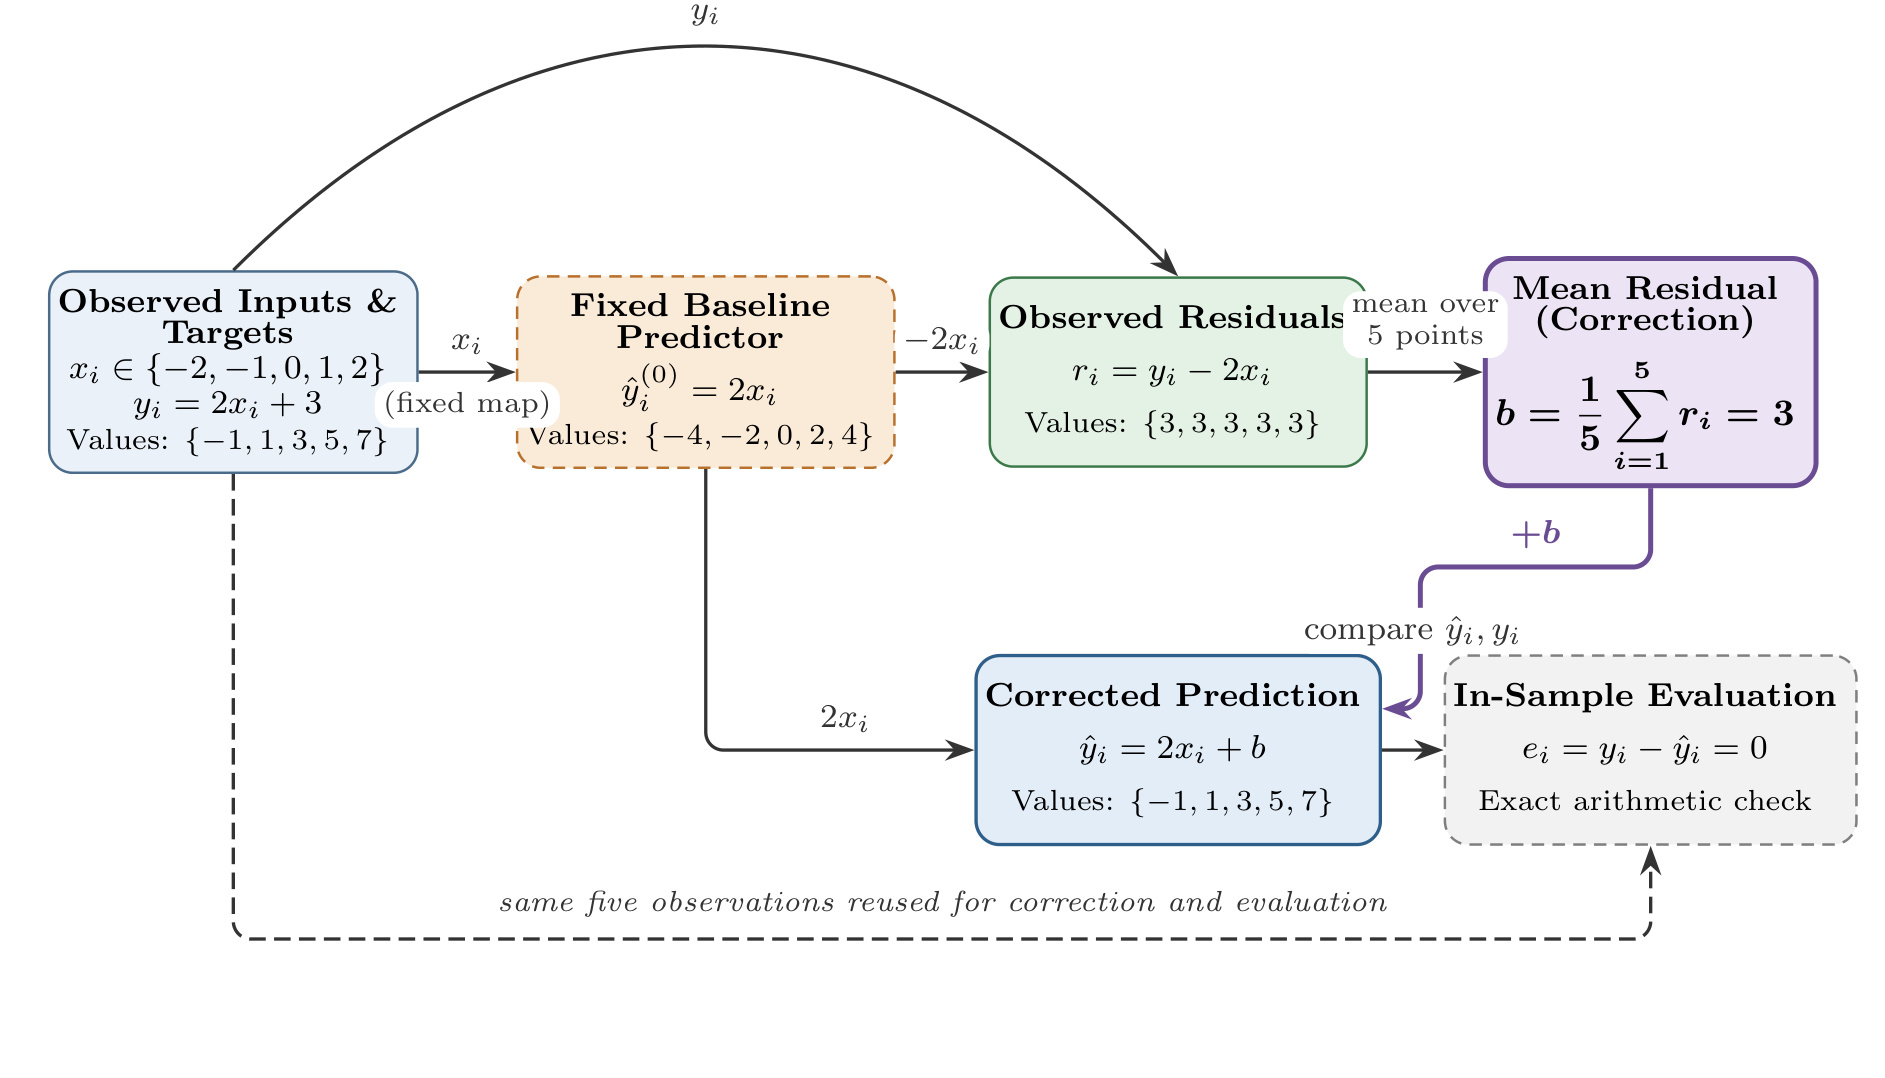
\includegraphics[width=\linewidth]{figures/fig_residual_workflow.jpg}
    \caption{Computational dependencies for the five supplied observations. Targets and baseline predictions determine residuals; their mean gives the least-squares intercept $b=3$. The dashed path identifies the same targets entering in-sample evaluation.}
    \label{fig:residual_workflow}
\end{figure}

\section{Experiments}

\subsection{Observations and Evaluation Protocol}

The supplied experimental log documents one deterministic base R calculation. All five observations determine the mean residual and evaluate the settings $b=0,1.5,3$. The slope remains fixed throughout. The setting $b=0$ represents the original predictor, $b=1.5$ illustrates a halfway correction, and $b=3$ is the fitted least-squares intercept.

These settings describe three scalar choices within one calculation. The computation reproduces the algebraic results, and its evaluation is explicitly on the fitting observations. This protocol makes the provenance of zero error directly traceable.

\subsection{Recorded Errors and Reproducible Figures}

Table~\ref{tab:recorded_errors} retains the values supplied by the R calculation. Their exactness follows from the constant residual construction. At $b=1.5$, each residual is half its baseline value: MAE is therefore halved, whereas MSE becomes one quarter of its baseline value. At $b=3$, every residual vanishes.

\begin{table}[htbp]
    \centering
    \caption{Errors reproduced by R and determined algebraically on the five fitting observations.}
    \label{tab:recorded_errors}
    \begin{tabular}{rrr}
        \toprule
        Added $b$ & Mean absolute error & Mean squared error \\
        \midrule
        0   & 3   & 9    \\
        1.5 & 1.5 & 2.25 \\
        3   & 0   & 0    \\
        \bottomrule
    \end{tabular}
\end{table}

Figure~\ref{fig:intercept_error} provides a visual reading of these same three MSE values. Its supplied title uses ``Measured'' for the deterministic computational check of the exact expressions. The table supports numerical comparison, while the plot emphasizes the different squared-error levels.

An instructional check is to ask readers to derive the middle table row before consulting the plot, then trace the evaluation targets backward through the flow diagram. Together, these tasks connect numerical calculation with interpretation of the evaluation protocol.

\begin{figure}[htbp]
    \centering
    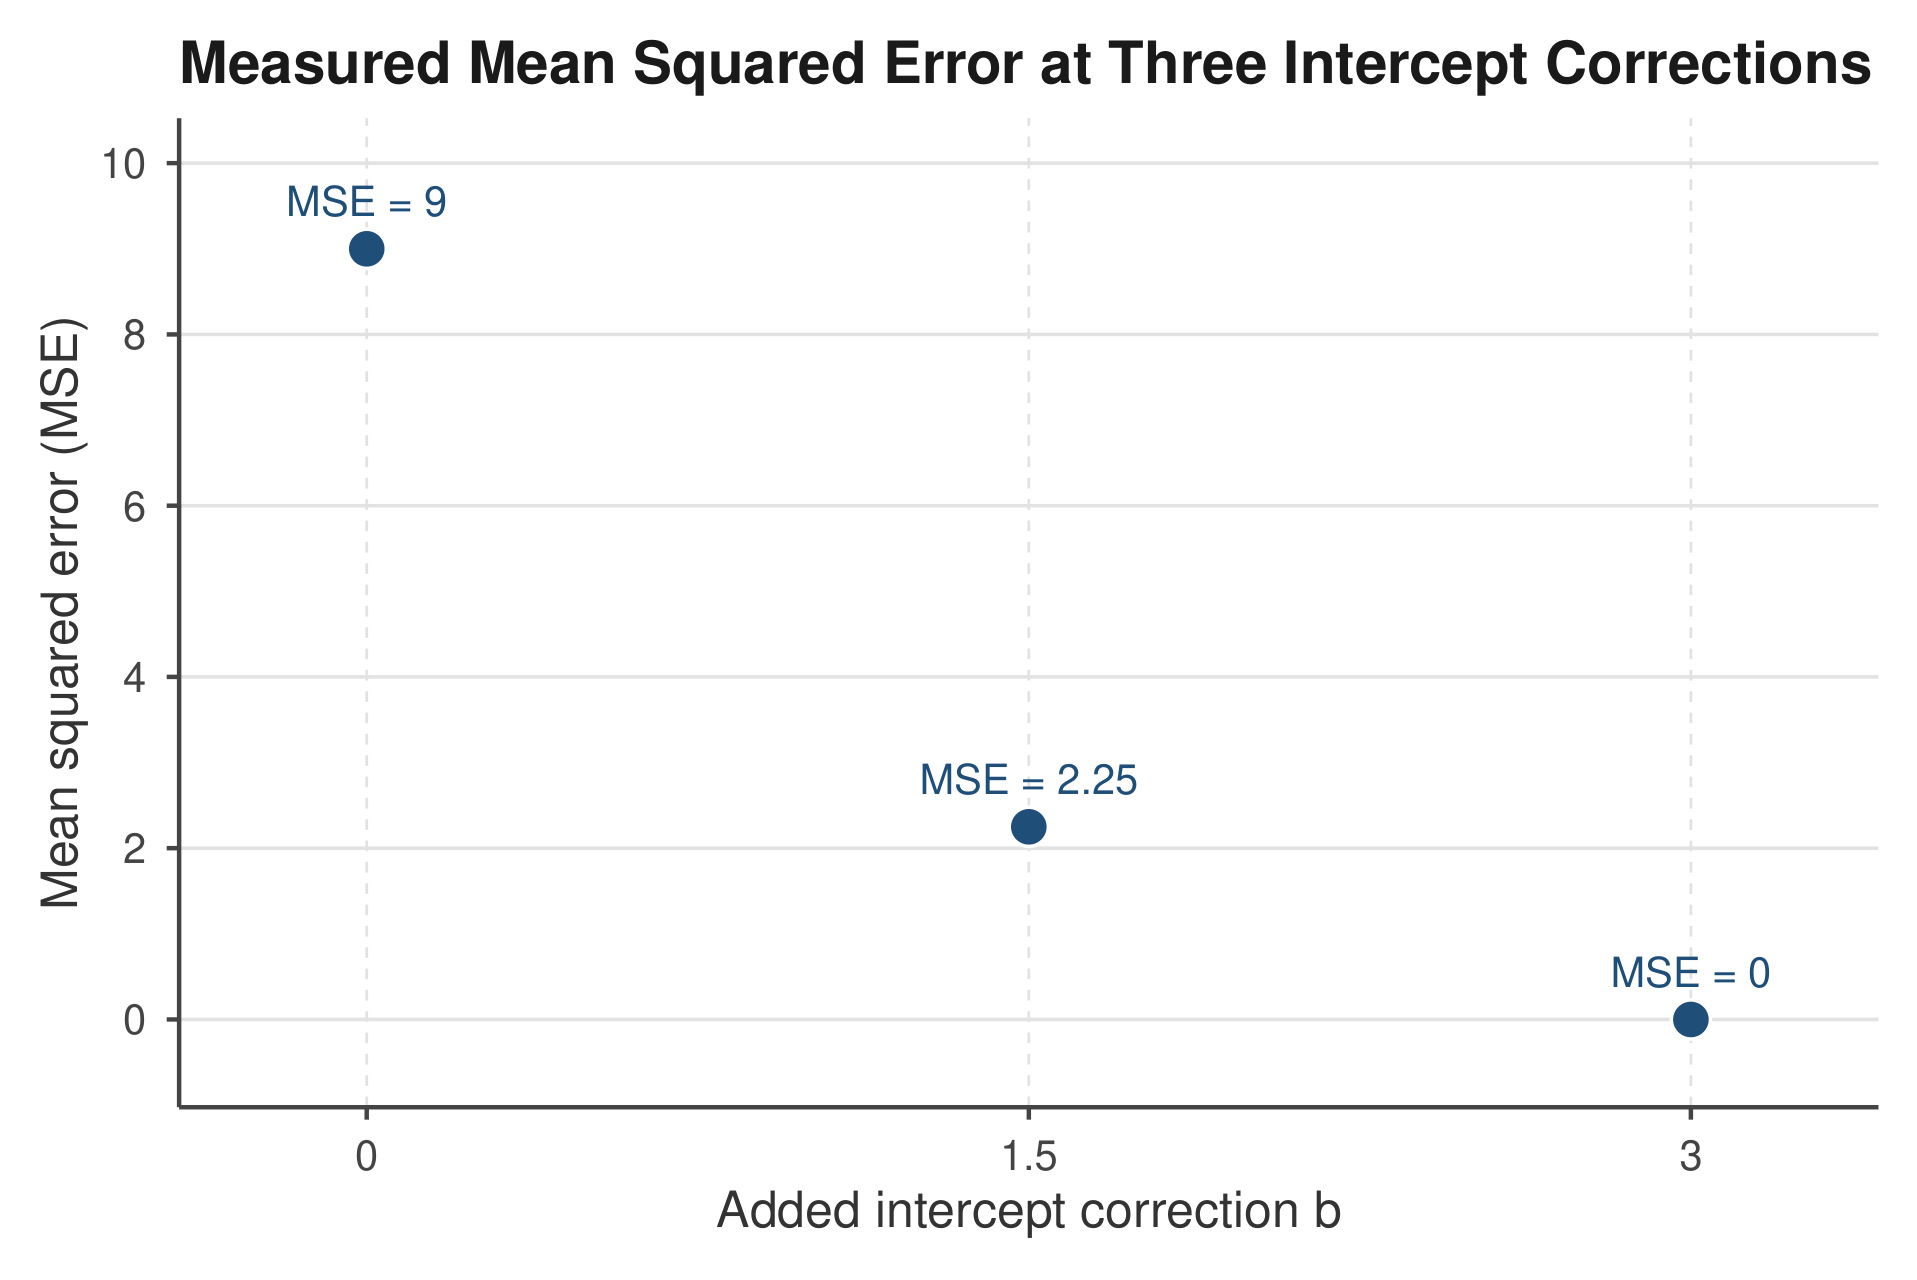
\includegraphics[width=\linewidth]{figures/fig_intercept_error.jpg}
    \caption{The three supplied computational checks:
    $(b,\operatorname{MSE})=(0,9),(1.5,2.25),(3,0)$.
    Each value follows exactly from $(3-b)^2$ on the five fitting observations.}
    \label{fig:intercept_error}
\end{figure}

\section{Conclusion}

For a fixed baseline predictor, the mean residual is the least-squares intercept correction. In the supplied constant-residual example, $b=3$ reproduces all five targets and makes both error summaries zero. The lesson combines a finite least-squares derivation, exact computational checks, and an explicit account of observation reuse. Its central learning outcome is to interpret the fitting operation and its resulting errors together.


\begin{thebibliography}{9}

\bibitem{Eisenhauer2003RegressionThrough}
Joseph G. Eisenhauer.
\newblock Regression through the Origin.
\newblock \emph{Teaching Statistics}, 2003.

\bibitem{Gneiting2011MakingEvaluating}
Tilmann Gneiting.
\newblock Making and Evaluating Point Forecasts.
\newblock \emph{Journal of the American Statistical Association}, 2011.

\bibitem{Efron1986HowBiased}
Bradley Efron.
\newblock How Biased is the Apparent Error Rate of a Prediction Rule?
\newblock \emph{Journal of the American Statistical Association}, 1986.

\end{thebibliography}

% PAPER_ORCHESTRA_PROVENANCE_BEGIN
\clearpage
\section*{Figure source provenance}
The files below are the exact sources that produced the embedded figure previews. Paths are relative to this manuscript's source directory. The accompanying \texttt{figure\char95{}provenance.json} records all artifact checksums.\par
\medskip\noindent\textbf{Figure~\ref{fig:intercept_error} (\texttt{fig\char95{}intercept\char95{}error.jpg}).}\par
\noindent R/ggplot2 source: \texttt{figure\char95{}code/\allowbreak{}fig\char95{}intercept\char95{}error/\allowbreak{}source.R}.\par
\noindent Source SHA256: \texttt{2479e40e\allowbreak{}8d39e8e1\allowbreak{}6c29f883\allowbreak{}7e3b8df9\allowbreak{}909f9f65\allowbreak{}8bb35b95\allowbreak{}9fda0b12\allowbreak{}96debbe4}.\par
\noindent Rendering metadata: \texttt{figure\char95{}code/\allowbreak{}fig\char95{}intercept\char95{}error/\allowbreak{}render.json}.\par
\noindent Exact export wrapper: \texttt{figure\char95{}code/\allowbreak{}fig\char95{}intercept\char95{}error/\allowbreak{}worker.R}.\par
\noindent Wrapper SHA256: \texttt{1aedad4b\allowbreak{}1547d4b2\allowbreak{}d394cbb0\allowbreak{}239655d3\allowbreak{}667d453d\allowbreak{}d1fd0eca\allowbreak{}3e77c037\allowbreak{}e6d34892}.\par
\noindent Rendering metadata: \texttt{figure\char95{}code/\allowbreak{}fig\char95{}intercept\char95{}error/\allowbreak{}sessionInfo.txt}.\par
\medskip\noindent\textbf{Figure~\ref{fig:residual_workflow} (\texttt{fig\char95{}residual\char95{}workflow.jpg}).}\par
\noindent LaTeX/TikZ source: \texttt{figure\char95{}code/\allowbreak{}fig\char95{}residual\char95{}workflow/\allowbreak{}source.tex}.\par
\noindent Source SHA256: \texttt{84e305cc\allowbreak{}09efdeb2\allowbreak{}bc2162c3\allowbreak{}9fc60cb1\allowbreak{}d1a3c538\allowbreak{}4254d368\allowbreak{}dee04e8d\allowbreak{}b66664b4}.\par
\noindent Rendering metadata: \texttt{figure\char95{}code/\allowbreak{}fig\char95{}residual\char95{}workflow/\allowbreak{}render.json}.\par
% PAPER_ORCHESTRA_PROVENANCE_END
\end{document}